%iffalse
\let\negmedspace\undefined
\let\negthickspace\undefined
\documentclass[journal,12pt,onecolumn]{IEEEtran}
\usepackage{cite}
\usepackage{amsmath,amssymb,amsfonts,amsthm}
\usepackage{algorithmic}
\usepackage{graphicx}
\usepackage{textcomp}
\usepackage{xcolor}
\usepackage{txfonts}
\usepackage{listings}
\usepackage{enumitem}
\usepackage{enumitem,multicol}
\usepackage{mathtools}
\usepackage{gensymb}
\usepackage{comment}
\usepackage[breaklinks=true]{hyperref}
\usepackage{tkz-euclide} 
\usepackage{listings}
\usepackage{gvv}                                        
%\def\inputGnumericTable{}                                 
\usepackage[latin1]{inputenc}                                
\usepackage{color}                                            
\usepackage{array}                                            
\usepackage{longtable}                                       
\usepackage{calc}                                             
\usepackage{multirow}                                         
\usepackage{hhline}                                           
\usepackage{ifthen}                                           
\usepackage{lscape}
\usepackage{tabularx}
\usepackage{array}
\usepackage{float}
\usepackage[american,siunitx]{circuitikz}
\usetikzlibrary{arrows,shapes,calc,positioning}
\usepackage{pgfplots}


\newtheorem{theorem}{Theorem}[section]
\newtheorem{problem}{Problem}
\newtheorem{proposition}{Proposition}[section]
\newtheorem{lemma}{Lemma}[section]
\newtheorem{corollary}[theorem]{Corollary}
\newtheorem{example}{Example}[section]
\newtheorem{definition}[problem]{Definition}
\newcommand{\BEQA}{\begin{eqnarray}}
\newcommand{\EEQA}{\end{eqnarray}}
\newcommand{\define}{\stackrel{\triangle}{=}}
\theoremstyle{remark}
\newtheorem{rem}{Remark}
\pgfplotsset{compat=1.18}

% Marks the beginning of the document
\begin{document}
\bibliographystyle{IEEEtran}
\vspace{3cm}

\title{XE-2022}
\author{EE24Btech11022 - Eshan Sharma}
\maketitle

\renewcommand{\thefigure}{\theenumi}
\renewcommand{\thetable}{\theenumi}



\begin{enumerate}
\item A wooden cylinder (specific gravity $= 0.6$) of length $L$ and diameter $D$ floats in water (density $1000 \, \text{kg/m}^3$). Find out the minimum value of $D/L$ for which the cylinder floats with its axis vertical. \textit{(Round off to three decimal places)}\\

\item Consider a cart of mass $10 \, \text{kg}$ placed on an inclined plane (angle of inclination $60^\circ$ with horizontal) as shown in the figure. A turning vane of negligible weight is mounted on the cart. A horizontal steady water jet is issued from a stationary nozzle of area $0.1 \, \text{m}^2$ and strikes the turning vane as shown in the figure. The vane turns the jet downward parallel to the inclined plane. Find out the minimum jet velocity (in m/s) which will not allow the cart to come down. Neglect friction, consider density of water $= 1000 \, \text{kg/m}^3$ and acceleration due to gravity $= 10 \, \text{m/s}^2$. \textit{(Round off to two decimal places)}\\

\begin{center}
	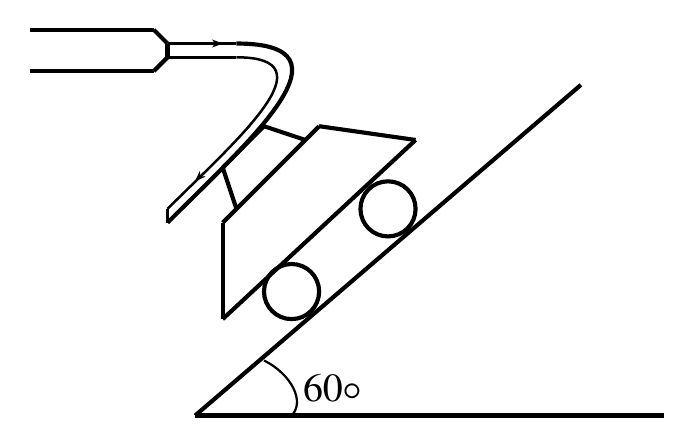
\begin{tikzpicture}[scale = 0.7]
		\tikzstyle{every node}=[font=\Large]
		\draw [line width=1.5pt, short] (8.75,8.75) -- (15.75,14.75);
		\draw [line width=1.5pt, short] (8.75,8.75) -- (17.25,8.75);
		\draw [ line width=1.5pt ] (10.5,11) circle (0.5cm);
		\draw [ line width=1.5pt ] (12.25,12.5) circle (0.5cm);
		\draw [line width=1.5pt, short] (9.25,10.5) -- (12.75,13.75);
		\draw [line width=1.5pt, short] (9.25,10.5) -- (9.25,12.25);
		\draw [line width=1.5pt, short] (9.25,12.25) -- (11,14);
		\draw [line width=1.5pt, short] (11,14) -- (12.75,13.75);
		\draw [line width=0.8pt, short] (10,9.75) .. controls (10.5,9.5) and (10.75,9) .. (10.5,8.75);
		\draw [line width=1.5pt, short] (9.25,13.25) -- (9.5,12.5);
		\draw [line width=1.5pt, short] (9.25,13.25) -- (10,14);
		\draw [line width=1.5pt, short] (10,14) -- (10.75,13.75);
		\draw [line width=1.5pt, short] (8.25,12.25) .. controls (9.75,13.75) and (11.75,15.5) .. (9.5,15.5);
		\draw [line width=1.5pt, short] (5.75,15.75) -- (8,15.75);
		\draw [line width=1.5pt, short] (8,15.75) -- (8.25,15.5);
		\draw [line width=1.5pt, short] (8.25,15.5) -- (8.25,15.25);
		\draw [line width=1.5pt, short] (8.25,15.25) -- (8,15);
		\draw [line width=1.5pt, short] (8,15) -- (5.75,15);
		\node [font=\Large] at (11.25,9.25) {60$\circ$};
		\draw [line width=0.9pt, short] (8.25,12.5) .. controls (9.5,13.75) and (11.25,15.25) .. (9.5,15.25);
		\draw [line width=0.9pt, short] (8.25,15.5) -- (9.5,15.5);
		\draw [line width=0.9pt, short] (8.25,15.25) -- (9.5,15.25);
		\draw [line width=0.9pt, short] (8.25,12.5) -- (8.25,12.25);
		\draw [line width=0.2pt, ->, >=Stealth] (8.5,15.5) -- (9.25,15.5);
		\draw [line width=0.2pt, ->, >=Stealth] (9.75,14) -- (8.75,13);
	\end{tikzpicture}
\end{center}

\item A siphon is used to drain out water (density $1000 \, \text{kg/m}^3$) from a tank as shown in the figure. What can be the maximum height $z$ (in meters) of the point $C$? Consider acceleration due to gravity $= 10 \, \text{m/s}^2$, pressure at point $A = 101 \, \text{kPa}$, vapor pressure of water $= 29.5 \, \text{kPa}$, and neglect friction. \textit{(Round off to two decimal places)}\\

\begin{center}
	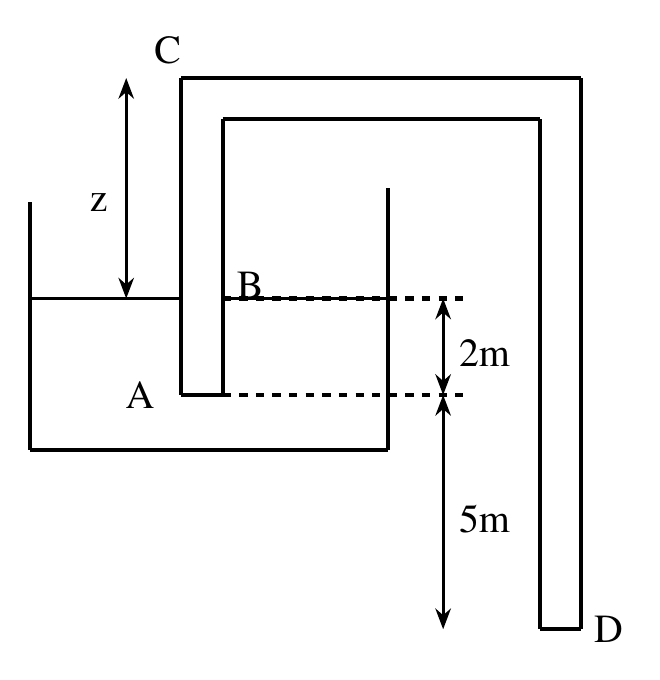
\begin{tikzpicture}[scale = 0.7]
		\tikzstyle{every node}=[font=\Large]
		\draw [line width=1.5pt, short] (6.5,13.25) -- (6.5,8.75);
		\draw [line width=1.5pt, short] (13,13.5) -- (13,8.75);
		\draw [line width=1.5pt, short] (6.5,8.75) -- (13,8.75);
		\draw [line width=1.5pt, short] (9.25,14.75) -- (9.25,9.75);
		\draw [line width=1.5pt, short] (10,14.75) -- (10,9.75);
		\draw [line width=1.5pt, short] (9.25,9.75) -- (10,9.75);
		\draw [line width=1.5pt, short] (10,14.75) -- (15.75,14.75);
		\draw [line width=1.5pt, short] (15.75,14.75) -- (15.75,5.5);
		\draw [line width=1.5pt, short] (15.75,5.5) -- (16.5,5.5);
		\draw [line width=1.5pt, short] (16.5,5.5) -- (16.5,15.5);
		\draw [line width=1.5pt, short] (16.5,15.5) -- (9.25,15.5);
		\draw [line width=1.5pt, short] (9.25,15.5) -- (9.25,14.75);
		\draw [line width=1.5pt, dashed] (10,9.75) -- (14.5,9.75);
		\draw [line width=1.5pt, dashed] (10,11.5) -- (14.5,11.5);
		\draw [line width=1pt, short] (6.5,11.5) -- (9.25,11.5);
		\draw [line width=1pt, short] (10,11.5) -- (13,11.5);
		\draw [line width=1pt, <->, >=Stealth] (14,9.75) -- (14,5.5);
		\draw [line width=1pt, <->, >=Stealth] (14,11.5) -- (14,9.75);
		\draw [line width=1pt, <->, >=Stealth] (8.25,15.5) -- (8.25,11.5);
		\node [font=\Large] at (8.5,9.75) {A};
		\node [font=\Large] at (10.5,11.75) {B};
		\node [font=\Large] at (9,16) {C};
		\node [font=\Large] at (17,5.5) {D};
		\node [font=\Large] at (7.75,13.25) {z};
		\node [font=\Large] at (14.75,10.5) {2m};
		\node [font=\Large] at (14.75,7.5) {5m};
	\end{tikzpicture}
\end{center}

\item The horizontal belt of negligible weight shown in the figure moves with a steady velocity $V$ of 2.5 m/s and skims over the top surface of an oil film of depth $h = 3$ cm. The length $L$ and width $b$ of the belt are, respectively, 2 m and 60 cm. Find the viscosity of the oil (in Pa-s), given that the minimum power required to move the belt is 100 W. Neglect the end effects.
\textit{(Round off to two decimal places)} \\ 

\begin{center}
	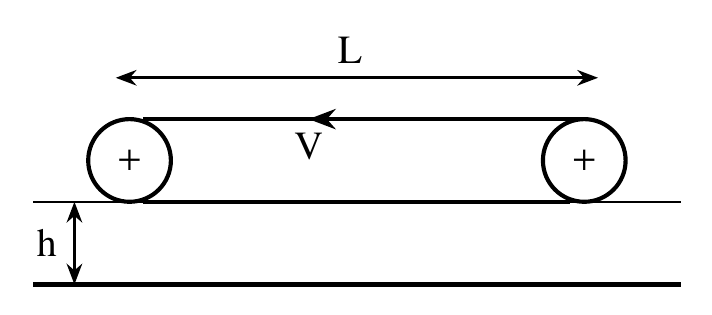
\begin{tikzpicture}[scale = 0.7]
		\tikzstyle{every node}=[font=\Large]
		\draw [line width=0.8pt, short] (7.5,11.75) -- (19.25,11.75);
		\draw [ line width=1.5pt ] (9.25,12.5) circle (0.75cm);
		\draw [ line width=1.5pt ] (17.5,12.5) circle (0.75cm);
		\draw [line width=1.5pt, short] (9.5,11.75) -- (17.25,11.75);
		\draw [line width=1.5pt, short] (9.5,13.25) -- (17.5,13.25);
		\draw [line width=2pt, short] (7.5,10.25) -- (19.25,10.25);
		\draw [line width=1.5pt, ->, >=Stealth] (14.25,13.25) -- (12.5,13.25);
		\draw [line width=1pt, <->, >=Stealth] (9,14) -- (17.75,14);
		\draw [line width=1pt, <->, >=Stealth] (8.25,11.75) -- (8.25,10.25);
		\node [font=\Large] at (13.25,14.5) {L};
		\node [font=\Large] at (7.75,11) {h};
		\node [font=\Large] at (12.5,12.75) {V};
		\node [font=\Large] at (9.25,12.5) {+};
		\node [font=\Large] at (17.5,12.5) {+};
	\end{tikzpicture}
\end{center}

\item Number of atoms per unit area of the (110) plane of a body-centered cubic crystal, with lattice parameter $a$, is

\begin{enumerate}
	\item $\frac{1}{a^2}$
	\item $\frac{\sqrt{2}}{a^2}$
	\item $\frac{1}{\sqrt{3}a^2}$
	\item $\frac{1}{\sqrt{2}a^2}$
\end{enumerate}

\item Match the following materials with their corresponding bonding types.

\begin{table}[ht!]
	\centering
	\resizebox{0.4\textwidth}{!}{
		\begin{tabular}[20pt]{ |c|c|c|c|c| }
    \hline
    \textbf{Activity} & \textbf{A} & \textbf{B} & \textbf{C} & \textbf{D} \\
    \hline
    \textbf{Mean(days)} & $6$ & $11$ & $8$ & $15$\\
    \hline 
    \textbf{Variance(days$^{2}$)} & $4$ & $9$ & $4$ & $9$\\
    \hline
\end{tabular}

	}
\end{table}

\begin{enumerate}
	\item P - 4; Q - 2; R - 3; S - 1
	\item P - 3; Q - 4; R - 2; S - 1
	\item P - 3; Q - 2; R - 1; S - 4
	\item P - 3; Q - 1; R - 4; S - 2
\end{enumerate}

\item In an ideal rubber, the primary factor responsible for elasticity up to small strains is
\begin{enumerate}
	\item Change in both enthalpy and entropy
	\item Change in enthalpy, but no change in the entropy
	\item No change in enthalpy, but change in the entropy
	\item Neither a change in enthalpy, nor a change in the entropy
\end{enumerate}

\item Which one of the following statements is true for an intrinsic semiconductor?
\begin{enumerate}
	\item Electrical conductivity increases with increasing temperature and pressure
	\item Electrical conductivity increases with increasing temperature and decreasing pressure
	\item Electrical conductivity increases with decreasing temperature and increasing pressure
	\item Electrical conductivity increases with decreasing temperature and pressure
\end{enumerate}

\item A differential scanning calorimetry (DSC) experiment tracks the heat flow into or out of a system as a function of temperature. If the experiments given in the options below are performed at 1 atmospheric pressure, then in which case will the DSC thermogram exhibit a spike, either upward or downward?
\begin{enumerate}
	\item Heating 10 mg of pure Cu from 323 K to 673 K
	\item Cooling pure water from 323 K to 278 K
	\item Heating pure ice from 263 K to 284 K
	\item Cooling a Pb-Sn alloy at the eutectic composition from 323 K to 273 K
\end{enumerate}

\item Which one of the following solvent environments will likely result in swelling of solid polystyrene?
\begin{enumerate}
	\item 0.1 M NaOH in H$_2$O
	\item HCl (aq.) of pH = 6
	\item Distilled water
	\item Benzene
\end{enumerate}

\item Vickers microhardness (HV) of a ductile material A is higher than another ductile material B. Which of the following is/are true?
\begin{enumerate}
	\item Young's modulus of A is greater than B
	\item Yield strength of A is greater than B
	\item Scratch resistance of A is greater than B
	\item Ductility of A is greater than B
\end{enumerate}

\item The enthalpy required to create an oxygen vacancy in CeO$_2$ is 4 eV. The number of oxygen vacancies present per mole of CeO$_2$ at 1000 K is \_\_\_\_\_\_\_.
(Round off to the nearest integer)

Given:
\begin{itemize}
	\item $N_A$: Avogadro's number = $6.02 \times 10^{23}$ mol$^{-1}$
	\item $k_B$: Boltzmann?s constant = $8.62 \times 10^{-5}$ eV/K
\end{itemize}

\item An electrochemical reaction is known to occur at +4.50 V against a Li$^+$/Li reference electrode. The potential of the same reaction against a Zn$^{2+}$/Zn reference electrode is \_\_\_\_\_\_\_ V. (Round off to two decimal places).

Given:
\begin{itemize}
	\item $E^0$ (Li$^+$/Li) = $-3.04$ V versus Standard Hydrogen Electrode
	\item $E^0$ (Zn$^{2+}$/Zn) = $-0.77$ V versus Standard Hydrogen Electrode
\end{itemize}

\end{enumerate}
\end{document}


